\chapter{Some More Stuff}
\label{cha:radon_trafo}




\begin{figure}[!h]
	\centering
	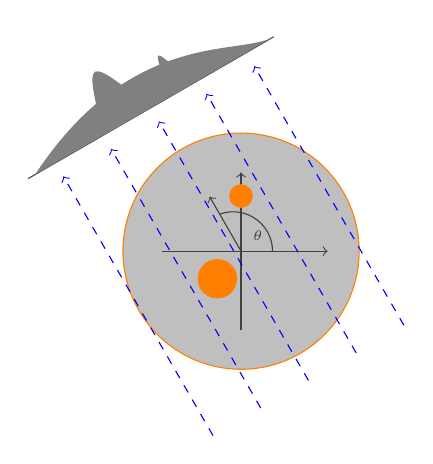
\begin{tikzpicture}[domain=3:3]  
	
	\fill[lightgray] (0.9,0) circle (1.5cm);
	
	\draw [darkgray] [->](-0.1,0) -- (2,0); % x-Achse
	%\draw (3, 0) node [right] {$x$};
	
	\draw [darkgray] [->](0.9,-1) -- (0.9,1); % y-Achse
	%\draw (0, 1.5) node [left] {$y$};
	
	%\draw (0.7, 0.2) node [right] {$\theta$};
	
	\draw [darkgray] [rotate=30, yshift=1.7cm](-1.1,0) -- (2.5,0); % s-Achse
	\draw [darkgray] [rotate=120, xshift=-1.45cm, yshift=-.78cm][->](1,0) -- (1.8,0); % s-Achse
	%\draw (1.4, 0)  node [yshift=3.7cm, right]    {$s$};
	%\draw  (0, 1.3) node [rotate=30, yshift=1.7cm] { Detektor};
	
	\draw [darkgray] (1.3,0) arc [start angle=0, end angle=110, radius=.5cm];
	\draw [darkgray](1.3, 0.2) node [left] {\tiny $\theta$};
	
	\fill[gray] [rotate=30, yshift=1.7cm] (-1,0) .. controls (1,1) and (2,0) .. (2.5,0);
	\fill[gray] [rotate=30, yshift=1.7cm] (0,0) .. controls (0.3,1)  .. (0.7,0);
	\fill[gray] [rotate=30, yshift=1.7cm] (1,0) .. controls (1.1,0.7)  .. (1.3,0);
	
	\draw[orange] (0.9,0) circle (1.5cm);
	\fill[orange] (0.9,  0.7) circle (.15cm);
	\fill[orange] (0.6, -0.35) circle (.25cm);
	%\draw (3.5, 1.1) node [left] {$f(x,y)$};
	
	%\draw[->] (0,0) -- (1.5, 0.7);
	%\draw (1.5, 0.7)  node [right] {$s$};
	
	\draw [rotate=30, dashed, ->] [blue] (0,-2.3) -- (0,1.5); % strahl
	\draw [rotate=30, xshift=-0.7cm, dashed, ->] [blue] (0,-2.3) -- (0,1.5); % strahl
	\draw [rotate=30, xshift=0.7cm, dashed, ->] [blue] (0,-2.3) -- (0,1.5); % strahl
	\draw [rotate=30, xshift=1.4cm, dashed, ->] [blue] (0,-2.3) -- (0,1.5); % strahl
	\draw [rotate=30, xshift=2.1cm, dashed, ->] [blue] (0,-2.3) -- (0,1.5); % strahl
	
	%\draw  (1.5,-1.4) node [rotate=30, yshift=-1cm, -] { Röntgenröhre};
	
	%\draw (1.55, -1.5)  node [right] {$I(s)$};
	%\draw (0.6, 1.7)  node [right] {$I(s + \Delta s)$};
	
	\begin{scope}[xshift=1cm]
	\end{scope}
	
	\end{tikzpicture}
	\caption{Schematischer Aufbau eines Computertomographen}
	\label{fig:5}
\end{figure}


\begin{figure}[!h]
	\centering
	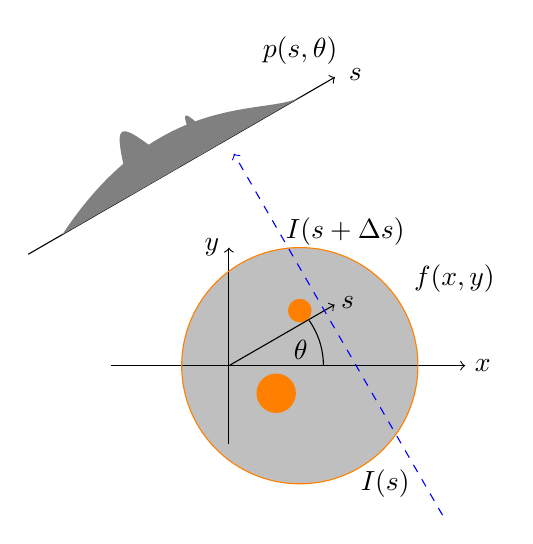
\begin{tikzpicture}[domain=3:3]  
	
	\fill[lightgray] (0.9,0) circle (1.5cm);
	
	
	\draw [->](-1.5,0) -- (3,0); % x-Achse
	\draw (3, 0) node [right] {$x$};
	
	\draw [->](0,-1) -- (0,1.5); % y-Achse
	\draw (0, 1.5) node [left] {$y$};
	
	\draw (0.7, 0.2) node [right] {$\theta$};
	
	\draw [rotate=30, yshift=2.5cm, ->](-1.5,0) -- (3,0); % s-Achse
	\draw (1.4, 0)  node [yshift=3.7cm, right]    {$s$};
	
	\draw (1.2,0) arc [start angle=0, end angle=35, radius=1cm];
	\draw (1.5, 4) node [left] {$p(s, \theta)$};
	
	\fill[gray] [rotate=30, yshift=2.5cm] (-1,0) .. controls (1,1) and (2,0) .. (2.5,0);
	\fill[gray] [rotate=30, yshift=2.5cm] (0,0) .. controls (0.3,1)  .. (0.7,0);
	\fill[gray] [rotate=30, yshift=2.5cm] (1,0) .. controls (1.1,0.7)  .. (1.3,0);
	
	\draw[orange] (0.9,0) circle (1.5cm);
	\fill[orange] (0.9,  0.7) circle (.15cm);
	\fill[orange] (0.6, -0.35) circle (.25cm);
	\draw (3.5, 1.1) node [left] {$f(x,y)$};
	
	\draw[rotate=30, ->] (0,0) -- (1.55, 0);
	\draw (1.3, 0.8)  node [right] {$s$};
	
	%\draw [rotate=30, dashed, ->] [blue] (0,-3) -- (0,2.3); % strahl
	%\draw [rotate=30, xshift=-0.7cm, dashed, ->] [blue] (0,-3) -- (0,2.3); % strahl
	%\draw [rotate=30, xshift=0.7cm, dashed, ->] [blue] (0,-3) -- (0,2.3); % strahl
	\draw [rotate=30, xshift=1.4cm, dashed, ->] [blue] (0,-3) -- (0,2.3); % strahl
	%\draw [rotate=30, xshift=2.1cm, dashed, ->] [blue] (0,-3) -- (0,2.3); % strahl
	
	\draw (1.55, -1.5)  node [right] {$I(s)$};
	\draw (0.6, 1.7)  node [right] {$I(s + \Delta s)$};
	
	
	\end{tikzpicture}
	
	\caption{Schematischer Aufbau eines Computertomographen}
	\label{fig:510}
\end{figure}

Radon\footnote{\label{foot:20} Johann Karl August Radon (1887-1956) österreichischer Mathematiker.}


\begin{equation}
	\begin{xy}
	\xymatrix{
		& L^2(\Omega) \ar@<2pt>[dl]_{\tilde{\mathcal{R}^*}} \ar@<2pt>[rd]^{\mathcal{R}} & \\
		L^2(Z, \frac{1}{\gamma(s)}) \ar@<2pt>[ru]_{\tilde{\mathcal{R}}} \ar@<2pt>[rr]^{\psi} &    & L^2(Z) \ar@<2pt>[lu]^{\mathcal{R}^*} \ar@<2pt>[ll]^{\psi^{-1}}
	}
	\end{xy}
\end{equation}




\newpage
\section{Anhang}

\begin{theorem}
	Der Satz von foo!
\end{theorem}
\begin{theorem}
	Der Satz von bar!
	\label{thm:foo}
\end{theorem}
\begin{proof}
	Beweis fertig.
\end{proof}
\begin{proof}[Beweis von Satz~\ref{thm:foo}]
	Beweis erbracht.
\end{proof}


\begin{Bemerkung}
	Der Satz von foo!
	
\end{Bemerkung}




